%%\textbf{}%%%%%%%%%%%%%%%%%%%%%%%%%%%%%%%%%%%%%%%%%%%%%%%%%%%%%%%%%%%%%%%%%%%%%%%%%%%%%%
%2345678901234567890123456789012345678901234567890123456789012345678901234567890
%        1         2         3         4         5         6         7         8
% THESIS CHAPTER


\chapter{C++ Code Scheme}
\label{chap:AppendixCode}
\ifpdf
\graphicspath{{Appendix/Figures/PNG/}{Appendix/Figures/PDF/}{Appendix/Figures/}}
\else
\graphicspath{{Appendix/Figures/EPS/}{Appendix/Figures/}}
\fi

Some effort has been spent to implement a flexible and modular C++ code architecture. The main focus is directed to facilitate the use of the TPIK approach. With this scheme, adding and removing tasks from the code is easy and straightforward. Furthermore, even if ROS is used as interface, other communication methods (for different simulators, or even for real robots) can be used easily, changing a little part of the code. This is due to the fact that all the ROS parts (the \textit{interface} classes) are written in separate files from the ones of the main blocks.\\
Only a rough idea about the code scheme is given here, without too much details. Further explanations can be found in the github page (\url{https://github.com/torydebra/AUV-Coop-Assembly}) and in the code documentation (\url{https://torydebra.github.io/AUV-Coop-Assembly/}).

\section{Tools}
The Control Architecture is implemented in C++ language. Some external support libraries have been used, and, in this section, the most relevant ones are described. Please note that a particular section (section \ref{sec:simulators}) is dedicated to the choice of the simulator, and another lists the main tools used by Vision (section \ref{sec:visionTools}).

\begin{itemize}
	\item \href{http://www.ros.org/}{\textbf{ROS}} (Robot Operating System), the well-known robotic middleware. It is used to communicate with the simulator, which means sending commands to robots and receiving information by the on-going simulations (e.g. robots states, data from sensors, streaming images from cameras).
	
	\item \href{http://eigen.tuxfamily.org/index.php?title=Main_Page}{\textbf{Eigen}} [\cite{eigen}], a C++ library for linear algebra. It is very useful to deal with matrix computation and management in any C++ software.
	
	\item \textbf{CMAT}, another C++ library, developed at GRAAL laboratory of University of Genova (\url{http://www.graal.dibris.unige.it/}). It implements the core functions for the TPIK method, detailed in \cite{IntroMaris1}.
	
	\item \href{http://www.orocos.org/kdl}{\textbf{Orocos KDL}}, a package to deal with kinematic and dynamic chains. Here it is used to compute the Jacobian of the robots, given the arm and the vehicle configuration.
\end{itemize}

\section{The single Robot Code Scheme}
\begin{figure}[H]
	\begin{center}
		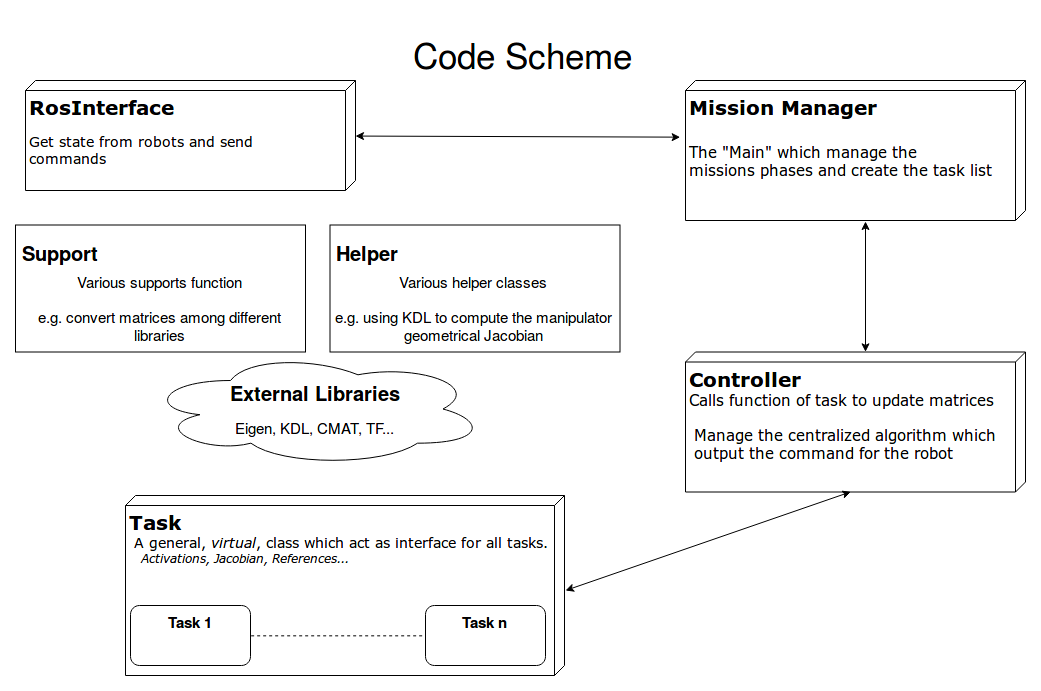
\includegraphics[width=1\columnwidth]{CodeScheme_single.png}
		\caption[C++ Code Scheme for the single robot]{The C++ code scheme that shows the relationship among the main blocks of the single robot. Parallelepipeds represent the principal blocks, while rectangles contain useful functions used by them. Arrows indicate the communication between the main blocks.}
		\label{fig:codeSchemeSingle}
	\end{center}
\end{figure}

In this section it is presented the scheme for the single carrying robot. The two cooperative robots share the same code, and they are differentiated (when necessary) thanks to their names (\textit{g500\_A} and \textit{g500\_B}).

\begin{itemize}
	\item \textbf{RosInterface}. This class is used to communicate with the simulator, e.g. sending commands to the robot, receiving state and sensor information, and so on. It is obviously ROS-dependent, and it should be replaced if another middleware is used.
	
	\item \textbf{Mission Manager}. This block is the \enquote{main}. It initializes all the useful classes, it creates the tasks list, and it manages the whole mission.
	
	\item \textbf{Controller}. This class is the core of the control; in practice it is the kinematic layer. It generates commands for the vehicle according to the prioritized list of tasks. It is where the iCAT algorithm based on the TPIK approach (section \ref{sec:tpik}) is used.
	
	\item \textbf{Task}. This is an \textit{abstract} class. It acts as a base class for all the specific \textit{concrete} classes of tasks. In this way, the controller and the mission manager simply handle a vector of pointer to Task. The Mission Manager creates a concrete class for each task and then it fills the vector. This vector is the prioritized list of the TPIK method. The controller can iterate the element of this vector and can call the abstract methods of Task without worrying of which real concrete task is actually inside the list.
	
	\item \textbf{Support}. It is a group of various \textit{namespaces}, used for conversions, to print to file, and to use some mathematical formulas.
	
	\item \textbf{Helper}. It contains a group of classes and headers used to help the control scheme (e.g. to compute the Jacobian with KDL) and to log results.
\end{itemize}


\section{The whole Code Scheme}
\begin{figure}[H]
	\begin{center}
		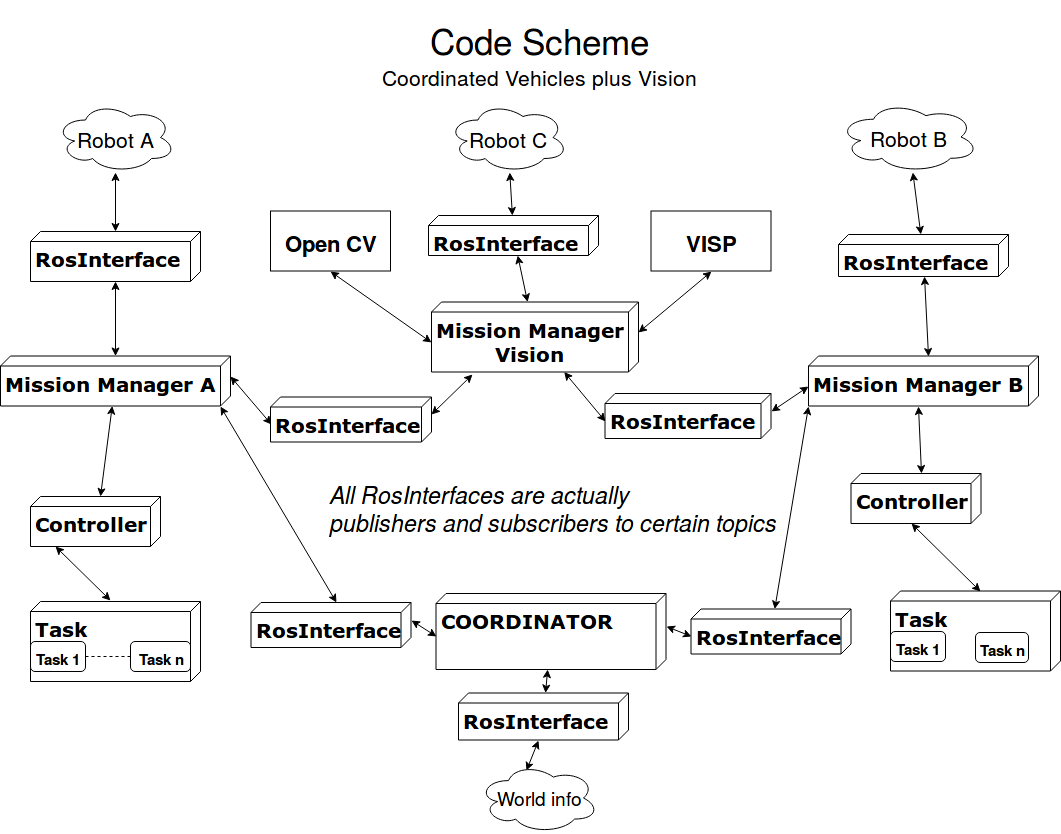
\includegraphics[width=1\columnwidth]{CodeScheme.png}
		\caption[C++ Code Scheme for the whole architecture]{The C++ code scheme that shows the relationship among the main blocks of the three robots. On the left and on the right side there is a zoomed out view of the previous figure \ref{fig:codeSchemeSingle}, corresponding to the scheme for the two carrying agents. In the centre, there are the blocks for the Vision robot and for the Coordinator.}
		\label{fig:codeSchemeWhole}
	\end{center}
\end{figure}
	
The two robots must communicate between them and with the Vision robot. Like explained before, ROS is used to communicate with the simulator, but it is also used to make different nodes (e.g. Coordinator and Robots) to communicate.\\
Please note that the Coordinator is not a physical agent: it can be put as a software routine on one robot. This would help with the communication issues typical of underwater scenarios, because only data-exchange between the Coordinator and the other robot will pass through the water.\\
The scheme for the Vision robot is simple because it is driven as a ROV: it is not autonomous and so no TPIK is implemented for it. Anyway, it can be switched easily into an autonomous robot, with or without TPIK (that it is not really necessary for this agent).\\
The Coordinator is a node in charge of dealing with the coordination policy explained in section \ref{sec:coopScheme}. It also needs information from the world (i.e. the simulation) to compute the cooperative velocity.
